\chapter { پیاده سازی }

در این بخش به روش‌ها و ابزارهای استفاده شده در پیاده‌سازی سیستم انیمیشن اشاره خواهد شد

\section {ابزارها}

\subsection {
    \lr{OpenGL}
    }

\lr{OpenGL}
یک واسط برنامه نویسی کاربردی  
\LTRfootnote{API}
است که با فراهم کردن توابع مختلف به توسعه‌دهندگان امکان دستکاری گرافیک و تصاویر را می‌دهد.
\lr{OpenGL} 
یک کتابخانه‌ی رندرینگ است.
یک "شئ" به خودی خود در
\lr{OpenGL} 
مفهومی ندارد
و به صورت مجموعه‌ای از مثلث‌ها و حالات مختلف درنظر گرفته می‌شود. بنابراین  
وظیفه‌ی ما است که بدانیم چه شئ‌ای در کدام قسمت صفحه رندر شده است. این کتابخانه تنها وظیفه‌اش، کشیدن تصاویری که است که می‌خواهیم به تصویر کشیده‌شوند.
در این صورت اگر می‌خواهیم تصویری را به‌روزرسانی کنیم و یا به عنوان مثال شئ‌ای را تحرک دهیم باید به 
\lr{OpenGL}
درخواست دهیم که صحنه را دوباره‌برای ما رندر کند.
\cite{KhronosUsingOpenGL}

به صورت کلی 
\lr{OpenGL}
را می‌توان یک ماشین حالت بزرگ درنظر گرفت. هر حالت شامل مجموعه‌ای از متغیر‌ها است که نحوه‌ی عملکرد
\lr{OpenGL}
را مشخص می‌کند. 
به مجموعه‌ی این حالت‌ها 
\lr{OpenGL context}
نیز می‌گویند. 
در واقع  
\lr{context}
را می‌توان یک شئ درنظر گرفت که کل
\lr{OpenGL}
را دربر می‌گیرد. عموما تمامی تغییرات، روی 
\lr{context}
فعلی اعمال می‌شود و سپس رندر می‌شود.
\cite{KhronosUsingOpenGL} \cite{LearnOpenGL_GettingStarted}

%%%%%%%%%%%%%%%%%%%%%%%%%%%%%%%%%%%%%%%%%%%%%%%%%%%%%

\subsection{\lr{GLFW}}

از آنجایی که به‌وجود‌آوردن یک پنجره‌ی جدید و همچنین 
\lr{context}
وابسته به نوع سیستم‌عامل است بنابراین نیازمند کتابخانه‌ای هستیم که بتواند این موارد را برای ما مدیریت کند.
\lr{GLFW}
یک کتابخانه‌ی منبع باز و چندپلتفرمی برای 
\lr{OpenGL}
است که یک
\lr{API}
ساده و مستقل از پلتفرم برای تولید پنجره‌ها، زمینه‌‌ها
\LTRfootnote{Contexts}
و سطوح، خواندن ورودی و مدیریت رویداد‌ها
\LTRfootnote{Events}
را ارائه می‌کند. 
این کتابخانه از سیستم‌عامل‌های 
ویندوز
، 
مک
و 
لینوکس
و سیستم‌های مشابه یونیکس پشتیبانی ‌می‌کند.
\cite{GLFW}


\subsection{\lr{GLAD}}
کتابخانه‌های گرافیکی مانند
\lr{OpenGL}
وظیفه‌‌ی پیاده‌سازی توابع گرافیکی را ندارند بلکه می‌توان آن‌ها را مانند یک هدر در زبان 
برنامه‌نویسی 
\lr{C++}
دانست که تعریف اولیه توابع را دارند. پیاده‌سازی این توابع در درایور‌های 
\lr{GPU}
قرار دارند.
دسترسی به این اشاره‌گر‌‌های تابع به خودی خود سخت نیست ولی از آنجایی که این اشاره‌گر ها وابسته به پلتفرم هستند بنابراین کار طاقت فرسایی است. 
وظیفه‌ی کتابخانه‌ی 
\lr{GLAD}
فراهم سازی و کنترل این اشاره‌گرهای تابع است.
\cite{GLAD}


\subsection{\lr{GLM}}
\lr{GLM}
یک کتابخانه‌ی ریاضی برای نرم‌افزارهای گرافیکی مبتنی بر زبان برنامه‌نویسی سایه‌ی 
\lr{OpenGL}
\LTRfootnote{OpenGL Shading Language(GLSL)} 
است. این کتابخانه تنها شامل یک هدر 
\lr{C++}
است.
توابع و کلاس‌های موجود در این کتابخانه به صورتی نامگذاری و طراحی شده‌آند که بسیار به 
\lr{GLSL}
 نزدیک باشند.


 \subsection{\lr{Assimp}}

 \lr{Assimp}
 یک کتابخانه برای بارگذاری و پردازش صحنه‌های هندسی از فرمت‌های مختلف است.
 می‌توان با استفاده از آن مواردی همچون مش‌های استاتیک و یا اسکلتونی، مواد 
 \LTRfootnote{Materials}
 ، انیمیشن های اسکلتونی و داده‌‌های بافت را از فایل بارگذاری کرد.
زمانی که این مدل‌ها بارگذاری می‌شوند این کتابخانه آن‌ها را در ساختاری به شکل زیر ذخیره می‌کند و بعد از آن می‌توان از این ساختار، داده‌های مورد نظر خود را خواند و از آن‌ها استفاده کرد.
\cite{Assimp} \cite{LearnOpenGL_Assimp}

\begin{figure}[ht]
	\centerline{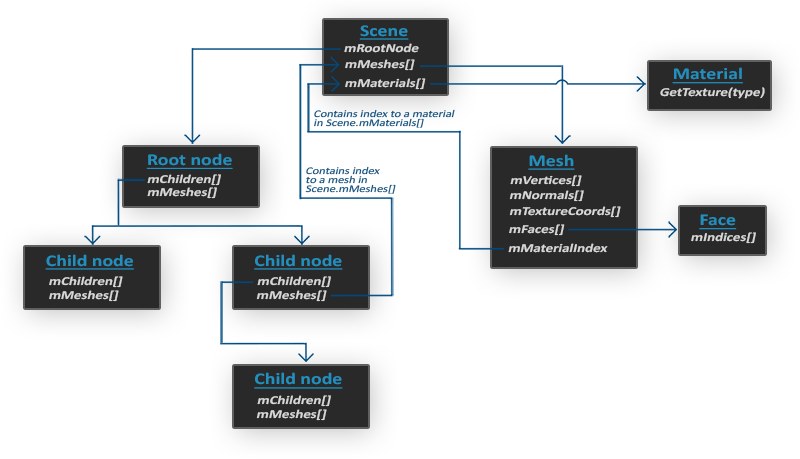
\includegraphics[width=\textwidth,height=\textheight,keepaspectratio]{Figures/Ch5/assimp_structure.png}}

	\caption{ساختار کلاس‌های کتابخانه‌ی \lr{Assimp} \cite{LearnOpenGL_Assimp}}
	\label{fig:Assimp}
  \end{figure}
  


  
\subsection{\lr{stb}}

این کتابخانه برای بارگذاری تصاویر استفاده می‌شود. در این پروژه از این کتابخانه برای بارگذاری
تصاویر بافت‌ها در کنار کتابخانه‌ی 
\lr{Assimp}
استفاده شده است.
\cite{stb}


\section{پیاده‌سازی}

این بخش دو هدف کلی را دنبال می‌کند.

\begin{enumerate}
	\item نمایش مدل گرافیکی و اجرای انیمیشن بر روی ‌آن
	\item ترکیب انیمیشن‌های مختلف به وسیله‌ی ماشین حالت

\end{enumerate}

\subsection{نمایش مدل گرافیکی}

همانطور که گفته شد مدل‌ها یا اشیاء سه‌بعدی به خودی خود مفهومی در 
\lr{OpenGL}
ندارند. آنچه برای 
\lr{OpenGL}
اهمیت دارد لیستی از مثلث‌ها است تا آن‌ها را به تصویر بکشد.
مدل‌های سه‌بعدی از رئوس، لبه و وجوه تشکیل می‌شوند و در فرمت‌های مختلفی مانند
\lr{FBX}
ذخیره می‌شوند. در این پیا‌ده‌سازی، از کتابخانه‌ی 
\lr{Assimp}
برای خواندن این داده‌ها استفاده شده است.

\subsection{قرارگیری مدل سه‌بعدی در کارت گرافیک}

آنچه برای 
\lr{OpenGL}
 اهمیت دارد این است که به آن مجموعه‌ای از مثلث‌ها داده شود تا برایمان ترسیم کند.
برای اینکار به صورت عمومی از 3 آرایه مختلف استفاده می‌شود که به نام‌های 
\lr{VBO}
،
\lr{VAO}
و 
\lr{EBO}
شناخته می‌شوند.
\lr{VBOs}
\LTRfootnote{Vertex Buffer Objectss}
یک آرایه یا بافری است که تمامی رئوس مدل سه‌بعدی ما را در خود جای می‌دهد.

همانطور که در بخش  2-2-1
اشاره شد، رئوس علاوه بر اینکه شامل اطلاعات موقعیت مکانی در محیط سه‌بعدی هستند، شامل اطلاعات دیگری 
نظیر رنگ، بردار نرمال، مختصات بافت  و... نیز می‌توانند باشند. بنابراین باید به صورتی به کارت گرافیک 
اعلام کنیم که این داده‌ای که در آرایه‌ی 
\lr{VBOs}
قرار دارد را چگونه تفسیر کند.
اینکار با استفاده از یک آرایه‌ی دیگر به نام 
\lr{VAO}
\LTRfootnote{Vertex Array Objects}
صورت می‌گیرد.
در نهایت گفتیم که آنچه برای کارت گرافیک اهمیت دارد دریافت مثلث‌ها است. بنابراین باید به طریقی بگوییم کدارم رئوس با 
اتصال به یکدیگر مثلث تشکیل می‌دهند. اینکار نیز با استفاده از آرایه‌ی 
\lr{EBOs}
\LTRfootnote{Element Buffer Objects}
صورت می‌گیرد.

\subsection{اسکلت شخصیت}

اسکلت یک شخصیت به صورت مجموعه‌ای از مفاصل که به صورت سلسله مراتبی به یکدگیر متصل‌اند، تعریف می‌شود.
در این پیاده‌سازی کلاس 
\lr{Bone}
نشان‌دهنده‌ی هر مفصل است.
هر 
\lr{Bone}
یک والد دارد و می‌تواند به هر تعدادی فرزند داشته باشد.
با توجه به تعریف آورده شده از اسکلت، کلاس اسکلت که با
\lr{Skeleton}
مشخص شده، شامل لیستی از این مفاصل به همراه اشاره‌گری به مفصل ریشه است.

\subsection{اتصال اسکلت و مدل سه‌بعدی}
اصطلاحی که برای اتصال اسکلت و مدل سه‌بعدی استفاده می‌شود
\lr{Skinning}
است.
در این روش هر راس موجود در مدل، به یک یا چند مفصل متصل می‌شود.
الگوریتم به کار‌رفته در این پیاده‌سازی،الگوریتم
\lr{linear blend skinning}
نام دارد. در این الگوریتم زمانی که یک راس به یک مفصل می‌شود به آن یک وزن نسبت داده می‌شود.
این وزن نشان‌دهنده‌ی میزان تاثیرگذاری این مفصل بر روی این راس است.
به بیانی دیگر، این وزن نشان می‌دهد که اکر این مفصل به مکان جدید منتقل شود، این انتقال چقدر بر روی آن راس تاثیر می‌گذارد.
بنابراین برای بدست آوردن انتقال نهایی راس، باید انتقال راس را نسبت به هرکدام از مفاصلی که به آن متصل است را بدست آوریم، سپس انتقال نهایی
برابر مجموع وزن‌دار تمامی این انتقال‌ها خواهد بود. 

\subsection{انیمیشن}
هر بازی‌های کامپیوتری هر کلیپ انیمیشنی شامل یک حرکت منحصر به فرد شخصیت داخل بازی است.
هر کلیپ‌ شامل ژست‌های اسکلت در فاصله‌های زمانی مشخصی است. در واقع آنچه باعث حرکت شخصیت می‌شود حرکت اسکلت شخصیت است.
زمانی که اسکلت شخصیت با استفاده از یک انیمیشن جابه‌جا می‌شود، مدل شخصیت نیز با استفاده از روش‌های 
\lr{skinning}
که در بالا توضیح داده‌شد همراه این اسکلت حرکت می‌کند.

انیمیشن‌ها از طریق کلاسی به اسم
\lr{Animation Clip}
مدل‌سازی شده اند. 
این کلاس شامل آرایه‌ای از ژست های شخصیت در مدت زمان‌های مشخصی است. همراه یک اشاره‌گری به اسکلت شخصیت.
نکته‌ی قابل توجه این است که هر کلیپ انیمیشنی مربوط به یک نوع اسکلت می‌شود. به زبانی دیگر نمی‌توان انیمیشنی که براس اسکلت
شخصیت انسانی طراحی شده است را بر روی یک حیوان، مانند فیل اجرا کرد.

\subsection{پخش‌کننده‌ی انیمیشن}

این سیستم وظیفه‌اش پخش کردن انیمیشن بر روی اسکلت شخصیت است.
این سیستم با گرفتن یک انیمیشن و یک اسکلت، این انیمیشن را بر روی آن اسکلت اجرا می‌کند.
همانطور که گفتیم، انیمیشن ها ژست شخصیت را در فاصله‌های زمانی مشخصی در خود ذخیره ‌می‌کنند. وظیفه‌ی این سیستم این است که با استفاده از یک زمان‌سنج که نشان‌دهنده‌ی زمان فعلی بازی است ژست مناسب شخصیت را از داخل انیمیشن بدست آورد.
قابل ذکر است که ممکن است این ژست با توجه به زمان بازی و فاصله‌های زمانی داخل انیمیشن
از درون‌یابی دو ژست پشت سر هم در آن کلیپ بدست آید.

\subsection{الگوریتم پخش‌کننده‌ی انیمیشن }

هر شخصیت درون بازی، اگر از نوع شخصیت اسکلتونی باشد، دارای یک پخش کننده ی انیمیشن خواهد بود.

در تصویر زیر تابع به‌روزرسانی اسکلت به وسیله‌ی انیمیشن را می‌توان مشاهده کرد.

\begin{latin}
	\begin{lstlisting}
		currentTime += deltaTime;

		const double currentAnimationTime = (currentTime - startTimeForCurrentAnim);
		AnimationPose currentPose = currentClip->GetPoseForCurrentFrame(currentAnimationTime * currentClip->GetFramePerSecond());
		
		SetSkeletonPose(currentPose);
	\end{lstlisting}
\end{latin}	



برای اینکه بتوان یک انیمیشن را پخش کرد نیاز است دو مورد زیر را بدانیم.

\begin{enumerate}
	\item زمان فعلی درون بازی(\lr{CurrentTime})
	\item زمان شروع پخش انیمیشن فعلی(\lr{StartTimeForCurrentAnimation}) 
\end{enumerate}

در ابتدا زمان فعلی درون بازی را برای این پخش‌کننده به‌روزرسانی می‌کنیم.
سپس برای بدست آوردن زمان فعلی انیمیشن می‌توان از فرمول زیر استفاده کرد

\lr{CurrentAnimationTime = CurrentTime - StartTimeForCurrentAnimation}

در نهایت با استفاده از این مقدار می‌توان ژست مورد نظر را از داخل کلیپ انیمیشنی بدست ‌آورد.
در نهایت نیز این ژست را بر روی اسکلت شخصیت اعمال می‌کنیم.


\subsection{ماشین حالت انیمیشن}

یکی از روش‌های ترکیب انیمیشن‌های مختلف با یکدیگر، استفاده از ماشین حالت متناهی است.
یک ماشین‌ حالت متناهی شامل چندی حالت مختلف است
که هر کدام از این حالات، حالتی از وضعیت سیستم را مشخص می‌کنند.
زمانی که از ماشین حالت استفاده می شود سیستم می‌تواند در هر لحظه تنها در یکی از این حالات قرار گیرد.
البته سیستم می‌تواند با دریافت ورودی از یک حالت به حالت دیگری رود.

دلیل استفاده از ماشین حالت متناهی برا سیستم انیمیشن این است که همانگونه که گفتیم، کلیپ‌های انیمیشنی، شامل ویدیو‌های کوتاهی هستند که یک حالت مشخصی از شخصیت را بیان می‌کنند.
در یک بازی، با توجه به ورودی بازیکن، شخصیت درون بازی می‌تواند در حالت‌های متفاوتی قرار گیرد. با استفاده از ماشین حالت می‌توان به تمامی این حالت‌ها رسیدگی کرد.

به عنوان مثال، تصویر زیر نشان‌دهنده‌ی یک ماشین‌حالت برای حرکت شخصیت است. شخصیت در ابتدا در حالت ایستاده قرار دارد و با گرفتن
ورودی‌های مختلف از کیبورد، می‌تواند به حالت‌های دیگری رود.

\begin{figure}[ht]
	\centerline{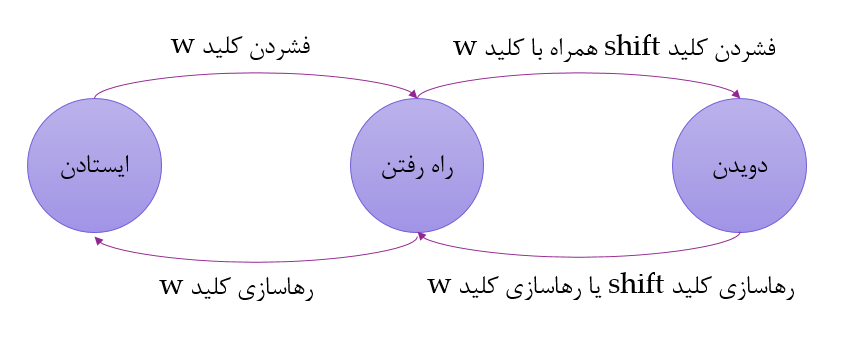
\includegraphics[width=\textwidth,height=\textheight,keepaspectratio]{Figures/Ch5/LocomotionStateMachine.png}}

	\caption{ماشین حالت برای حرکت شخصیت}
	\label{fig:LocomotionStateMachine}
\end{figure}


برای پیا‌ده‌سازی ماشین حالت متناهی، این سیستم به سه کلاس کلی شکسته‌شده‌است. کلاس
\lr{AnimationStateMachine}
که وظیفه‌ی مدیریت حالت‌ها و انتقال از یک حالت به حالت دیگری را دارد.
کلاس 
\lr{AnimationState}
که نشان‌دهنده‌ی حالت شخصیت است. هر 
\lr{AnimationState}
شامل یک کلیپ است و هر زمانی که این حالت فعال می‌شود این کلیپ پخش می‌شود.
 در نهایت کلاس
\lr{Transition}
که شامل توابع انتقال است.
هر حالت می‌تواند شامل چندین انتقال باشد. و وظیفه‌ی
\lr{AnimationStateMachine}
است که بررسی کند، اگر انتقالی امکان‌پذیر بود، آن را انجام دهد.

\subsection{به‌روزرسانی ماشین حالت انیمیشن}

وضعیت توابع انتقال تاثیرگذاری مستقیمی در وضعیت سیستم به‌روزرسانی ماشین حالت انیمیشن دارد.
وضعیت انتقال می‌تواند سه حالت زیر را داشته باشد.

\begin{enumerate}
	\item حالت عادی \LTRfootnote{Normal}
	\item حالت در حال انتقال \LTRfootnote{Transitioning}
	\item حالت اتمام انتقال \LTRfootnote{Finished}
\end{enumerate}


حالت اول حالت عادی
است که نشان‌دهنده‌ی وضعیت عادی ماشین حالت است. در این وضعیت، توابع انتقال حالت فعلی بررسی می‌شوند تا در صورتی که شرایطشان برقرار شود، تغییر حالت رخ دهد. علاوه بر آن انیمیشن حالت فعلی با استفاده از کلاس پخش‌کننده آپدیت می‌شود.

در صورتی که توابع انتقال مقدار درست
\LTRfootnote{True}
را بازگردانند، ماشین به وضعیت دوم که وضعیت درحال انتقال
است، تغییر وضعیت می‌دهد.
در این وضعیت با توجه به زمانی که مشخص شده، ژست شخصیت با استفاده از درون‌یابی خطی از حالت فعلی به حالت جدید تغییر می‌کند.

پس از اینکه انتقال به صورت کامل انجام شد، وضعیت ماشین حالت به اتمام انتقال
تغییر می‌یابد. زمانی که ماشین‌ در این وضعیت قرار گرفته یعنی به حالت جدید منتقل شده، بنابراین لازم است انیمیشن را از حالت جدید گرفته و آن را به کلاس پخش کننده داده تا آن را پخش کند.
پس از این کار وضعیت ماشین دوباره به حالت عادی تغییر می‌یابد و همه‌ی این موارد دوباره تکرار می‌شوند.

\begin{latin}
	

\begin{lstlisting}

	if(transitionStatus == TransitionStatus::normal) 
	{
		for (const auto&  transition : currentState->GetTransitions()) // loop through transitions of the current state
		{
			if (transition->Evaluate())
			{
				transitionStatus = TransitionStatus::transitioning;
				currentState = animationStatesMap.at(transition->to);
				TransitionFromPose = animator->GetPoseAtCurrentTime();
				TransitionToPose = currentState->GetAnimClip()->GetPoseForCurrentFrame(0);
				currentTime = 0;
				transitionTime = transition->transitionTime;
				break;
			}
		}
	}

	if (transitionStatus == TransitionStatus::normal)
	{
		animator->Update(deltaTime);
	}
	else if(transitionStatus == TransitionStatus::transitioning)
	{
		if(TransitionUpdate(deltaTime)) 
		{
			transitionStatus = TransitionStatus::finished;
		}
	}
	else if(transitionStatus == TransitionStatus::finished)
	{
		animator->ChangeAnimationClip(*(currentState->GetAnimClip()), 0); 
		transitionStatus = TransitionStatus::normal;
	}
\end{lstlisting}

\end{latin}